\chapter{Background \& Related Work}
\label{ch:Background}
This chapter first introduces important aspects of body temperature and then sensing with earables.
For body temperature, a distinction is made between core body temperature and skin temperature. 
In addition, the focus is on how temperature can be measured. 
In the subchapter on sensing with earables, the recording of data on the ear is generally introduced. 
Here a division of Röddiger \cite{roddigerSensingEarablesSystematic2022a} is explained.

\section{Body Temperature}
\label{Background:BodyTemperature}
In medical practice, temperature is one of the most frequently measured physical quantities.
By measuring temperature, one gains information about the internal energy of an object.
From the biophysical point of view, temperature measurement determines the changes in physical quantities that occur in a thermodynamic system \cite{dolibogComparativeAnalysisHuman2022}.
Temperature can be expressed in different scales.
These include Celsius, Fahrenheit, Kelvin, and Rankine \cite{grodzinskyUnderstandingFeverBody2020}.
The human body temperature range is usually between $36.5-37.5^\circ C$ \cite{hutchisonHypothermiaTherapyTraumatic2008}, varies constantly and depends on many influencing factors such as gender, age, time of day, and many others \cite{sund-levanderNormalOralRectal2002}.
Likewise, the state of consciousness and emotions are a decisive factor that significantly influences the body temperature \cite{barbosaescobarTemperatureEmotions2021}.
Furthermore, the position at which body temperature is measured is crucial \cite{Physiologie9783137960072ZVAB}.
In order to keep the body temperature within the normal temperature range through internal and external factors, the body uses thermoregulation, through which the temperature is constantly adjusted by signals from the central nervous system.

\subsection{Thermal Regulation}
\label{Background:BodyTemperature:ThermalRegulation}
A vital body function is the possibility of regulation of the exchange of body heat \cite{grodzinskyUnderstandingFeverBody2020}.
Regulation occurs through a neural feedback system. 
In many body parts, sensory means detect cold and heat and transmit them via the central nervous system to the hypothalamus reacting to potential temperature adjustments by triggering physiological activity. 
This can be associated with a gain or loss of heat, which maintains body temperature.
Major players in regulating body temperature are the cardiovascular system, the sudomotor control system, and skeletal muscles. 
The goal is to maintain body temperature within the range of $35^\circ C$ to $41^\circ C$ \cite{pierauTemperatursensibilitaet2001}. 
An excessive increase in body temperature (hyperthermia or hyperpyrexia), in which temperature regulation is no longer working, must be treated as a medical emergency.
The same applies if the body temperature drops below $35^\circ C$.

\subsection{Core Body Temperature}
\label{Background:BodyTemperature:CBT}
Core body temperature is the temperature of the body's internal organs, such as the heart, liver, and brain, and is a commonly used indicator of human health and endurance performance.
Unlike the body core temperature, the body surface temperature is more easily influenced by the ambient temperature and therefore cannot reflect the changes inside the body as well as the body core temperature.
Core body temperature can be measured invasively rectally, orally (oesophagus), in the pulmonary artery (with the use of a catheter), or in the urinary bladder \cite{moranCoreTemperatureMeasurement2002a}.
However, the gold standard is different.
The core body temperature of a healthy human body differs almost little from the temperature of the blood flowing in the pulmonary artery \cite{krizanacFemoroiliacalArteryPulmonary2013, holtzclawMonitoringBodyTemperature1993}.
This is exactly what is used as the gold standard for measuring body core temperature \cite{krizanacFemoroiliacalArteryPulmonary2013, holtzclawMonitoringBodyTemperature1993, fulbrookCoreBodyTemperature1997, maxtonEstimatingCoreTemperature2004}.
However, this comes with a few critical points.
Measuring the temperature of the blood flowing in the pulmonary artery involves an invasive and risky procedure that requires the insertion of a pulmonary artery catheter \cite{yeohRevisitingTympanicMembrane2017}.
This is strongly recommended in a medical hospital and nowhere else.
All of the previously mentioned methods are not comfortable for humans when measuring over a long period of time in everyday life.

Body temperature can also be measured non-invasive.
The following methods are much more convenient, but the measurement accuracy suffers somewhat.
Measuring the body temperature non-invasive can be done on the axilla, the tympanic membrane, and the body surface \cite{moranCoreTemperatureMeasurement2002a}.
Usually, core body temperature is constant only in the body core and consequently cannot be determined outside only by temperature sensors \cite{niedermannPredictionHumanCore2014}.
Due to this, it is necessary to use several other values for the calculation of the core body temperature in order to approximate the true temperature value. 
These can include e.g. skin temperature and skin heat fluxes or the heart rate.
Niedermann achieved a root mean square deviation (rmsd) ranging from $0.28 ^\circ C$ to $0.34 ^\circ C$ for all environmental conditions in 2014 \cite{niedermannPredictionHumanCore2014}.
Therefore, a principal component analysis (PCA) was performed to extract uncorrelated variables that were subsequently used in a linear regression model. 
Six parameters, consisting of three skin temperatures, two skin heat currents, and heart rate, were selected as input variables to generate two principal components. 
The predictive power of these components for estimating core body temperature was evaluated using multiple regression analysis.

\subsection{Skin Temperature}
\label{Background:BodyTemperature:SkinTemperature}
Skin temperature is often used to measure body temperature.
Skin temperature in general is the result of a dynamic equilibrium between the heat released during metabolic processes and transferred to the skin layer by thermal conduction and convection, the heat extracted from the environment, and the heat transferred to the environment by radiation, convection, and evaporation \cite{dolibogComparativeAnalysisHuman2022}.
Various sensors are used to measure skin temperature. 
These include the infrared sensors, but also the thermistors. 
Both are equal for purposes of clinical electrodiagnostic readings.
Thermistors offer better responsiveness and sensitivity in measurements.
Infrared thermistors, on the other hand, are more convenient in terms of speed and maneuverability \cite{burnhamThreeTypesSkinSurface2006}.
Because the skin is exposed to external influences, temperature differences can quickly occur.
This can be caused by cold or warm ambient air, but also by rain or other influences.
Measurements on the skin that cannot be easily influenced, such as the armpits, are suitable here.

\subsection{Temperature Measurements}
\label{Background:BodyTemperature:TemperatureMeasurements}
% TODO: General Temperature measurements of the human body
In General, the temperature of a human body will be measured with a thermometer.
There are multiple techniques available on which the temperature value will be calculated. 
These are divided into contact and non-contact thermometers.
For a detailed overview, take a look at chapters \ref{Background:TemperatureSensors:OpticalTS} and \ref{Background:TemperatureSensors:ResistanceTD}.
Body temperature is often measured in the armpit, mouth, rectum, ear, or forehead.
The temperature in the armpit is typically $36.6^\circ C$, in the mouth $36.9^\circ C$, and $37.1^\circ C$ in the ear \cite{dolibogComparativeAnalysisHuman2022}.
% TODO: wie siehts bei Rectal aus?
The rectal temperature testing method is the most accurate of all measurements, while non-contact forehead thermometers are considered the least accurate, and measurements are taken with them should be confirmed by other methods.
The minimum value of the standard error for the above methods is $0.1^\circ C$ [9].
Ear readings are assumed to be of similar accuracy when compared to the rectal method, which is most commonly used in infants, the correct value is usually $37.1^\circ C$ \cite{dolibogComparativeAnalysisHuman2022}.

% Ear based temperature measeurements
Ear-based temperature measurement uses a sensor to measure the temperature of the ear canal. 
The approach has a number of advantages over other measurement positions.
First, it is a non-invasive measurement procedure, which allows measurement nearly inside the body with the least amount of hematoma.
Second, the measurement is much more promising compared to other non-invasive alternatives, where many factors can contribute to falsifying the final result \cite{ganioValidityReliabilityDevices2009, craigTemperatureMeasuredAxilla2000}. 
However, it is essential to note that the accuracy of temperature measurement may depend on factors such as the positioning of the thermometer and the presence of earwax or other obstructions in the ear canal.

% \subsubsection{Temperature Measurements on the Tympanic Membrane}
The tympanic membrane is a thin membrane that separates the middle ear from the external auditory canal. 
The artery called the external carotid artery runs near the external auditory canal and radiates heat, which is why measuring the temperature at the tympanic membrane has a promising chance of determining body temperature \cite{yeohRevisitingTympanicMembrane2017}.

Since measuring body temperature at the tympanic membrane is a non-invasive measurement method, it is already being investigated as a possible replacement for currently accepted methods.
This could be a safe and very convenient way of measuring core body temperature, but to date it is not de-facto due to unresolved problems.
These include the accuracy and stability compared to measurements at other locations \cite{maxtonEstimatingCoreTemperature2004, fulbrookCoreBodyTemperature1997, mumaComparisonRectalAxillary1991, rothAgreementRectalTympanic1996}.
Benzinger \cite{benzingerHeatRegulationHomeostasis1969, benzingerClinicalTemperatureNew1969, benzingerPhysicalHeatRegulation1959} first demonstrated the feasibility of tympanic membrane measurement as an indicator of core body temperature using a thermocouple temperature probe that engages the surface of the tympanic membrane with the ear canal sealed from the environment.
For this, Benzinger made measurements of tympanic membrane temperature obtained from his probe and measurement approach and showed them to be stable, reproducible, and responsive to thermal stresses of various types.
However, there are other studies at a later date that refute individual assumptions of this study.
McCaffrey et al. \cite{mccaffreyEffectHeadSkin1975} and Nielsen \cite{nielsenNaturalCoolingBrain1988} showed that head cooling reduces the body core temperature when measured with exactly the procedure of Benzinger.
McCaffrey et al. however, also showed that by heating and cooling localized regions of the head, infrared measurement of temperature at the tympanic membrane of human subjects was not proportionally affected by changes in head skin temperature.
This suggests a contradiction, which means that this method may not be a good predictor of core body temperature because it depends on other, as yet unknown, variables.
Brinnel and Cabanac \cite{brinnelTympanicTemperatureCore1989} and Sato et al. \cite{satoReexaminationTympanicMembrane1996}, however, provided data showing that measurements for this purpose are still reliable if the measurement point on the tympanic membrane is carefully chosen. 
Brinnel and Cabanac proposed that the lower anterior quarter of the tympanic membrane (Figure \ref{fig:tympanic_membrane_mp}) has a higher temperature on the surface of the tympanic membrane and temperature measurement from a point in this area is the least sensitive to head cooling.
\begin{figure}[t]
    \centering
    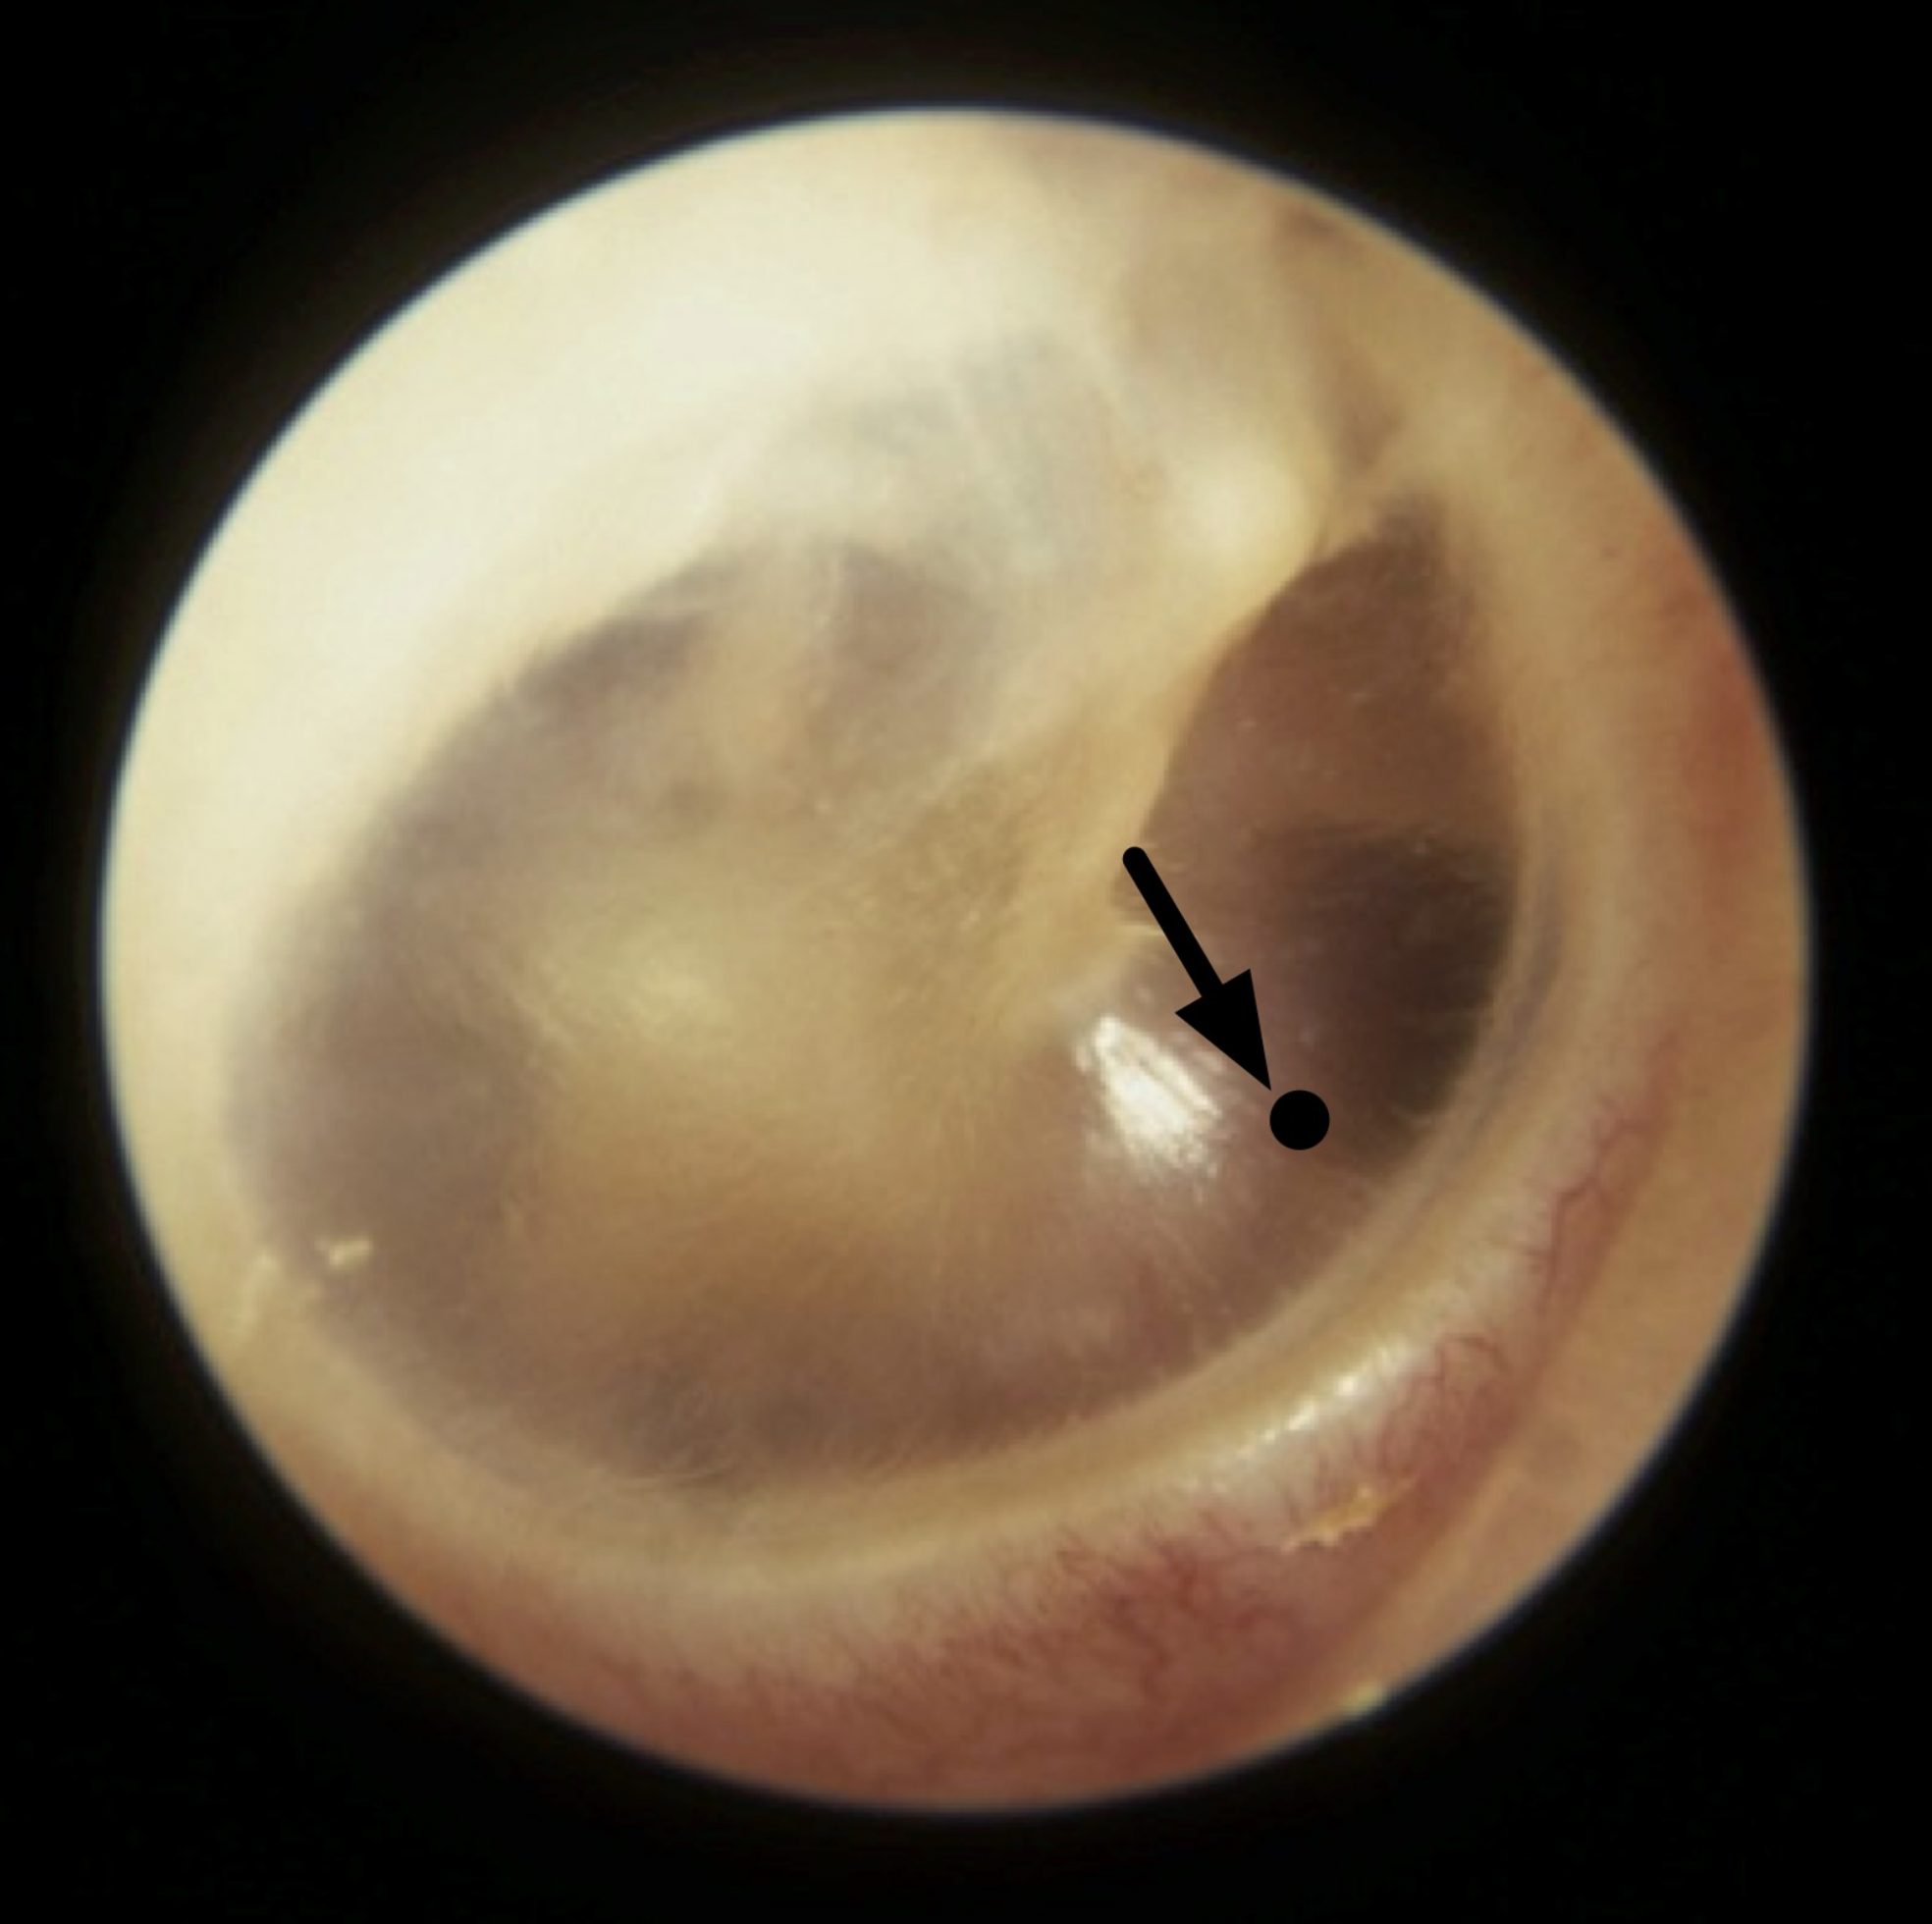
\includegraphics[scale=0.15]{thesis-doc/images/tympanic_membrane_mp.png}
    \caption{Measuring point on the tympanic membrane \cite{brinnelTympanicTemperatureCore1989}. Tympanic membrane of the right ear with a temperature measuring point in the lower front quarter (see arrow).}
    \label{fig:tympanic_membrane_mp}
\end{figure}

% das paper is von 1991, vllt schon zu alt und unrelevant
% TODO: \cite{ComparisonPulmonaryArtery}

% hier bei der comparison gehts um mittelohrentzündungen
% TODO: \cite{kimComparisonBilateralEardrum2022}

% das paper is von 1999, vllt schon zu alt und unrelevant
% TODO: \cite{childsTympanicMembraneTemperature1999}

Temperature sensors are used to measure the temperature of a particular object or environment.
They are widely used in many applications, such as industrial, medical, or scientific contexts.
Temperature sensors detect changes in temperature and convert this into a measurable signal.
There are various types of temperature sensors, including contact and non-contact sensors.
% Contact sensors
Contact sensors measure temperature by maintaining physical contact with an object and measuring the temperature there.
Contact sensors can be divided into 3 types: Thermocouples, Thermistors, and Resistance Temperature Detectors (RTDs). 
Thermocouples measure the voltage generated by two different metals when they are exposed to different temperatures.
RTDs measure changes in the electrical resistance of a metal wire when it has temperature changes.
Thermistors are semiconductor devices whose electrical resistance changes with temperature.
% Non-contact sensors
Non-contact sensors, on the other hand, do not require contact with the object being measured. They are also known as infrared sensors.
Non-contact sensors measure the emitted infrared radiation from an object and convert it into a measurable signal.
Most often, the sensors are used when contact with an object is not desirable or practical, such as can often be useful in a medical or scientific research context. 
This is also the case in this work, as contact with the tympanic membrane, for example, is not desired.
Non-contact sensors can be roughly divided into two categories: IR sensors and optical pyrometers.
IR sensors are devices that detect and measure the amount of infrared radiation emitted by an object. They operate on the principle that all objects emit infrared radiation in proportion to their temperature. 
Optical pyrometers, on the other hand, measure temperature by detecting the color of light emitted by an object. They work on the principle that the color of light emitted from a hot object changes as the temperature of the object changes.
However, the current classification here is very crude.
In addition to those mentioned above, there are, for example, fiber optic sensors and acoustic sensors.

When choosing the right sensor for a particular application, some things have to be considered.
Accuracy, response time, and range are important variables.
Depending on the requirement profile, the right sensor can be selected based on the parameters.
In the following, the optical temperature sensors, as well as the RTDs are described in more detail, since they are very important in this work.

\subsection{Optical Temperature Sensors}
\label{Background:TemperatureSensors:OpticalTS}
Optical temperature sensors, also known as optical pyrometers, measure temperature by detecting the color of light emitted from an object. 
This is based on the assumption that the color of the emitted light is different depending on the temperature.
Typically, this is done using a lens that focuses the emitted light from the object onto a detector, which then analyzes the color of the light. 
This is then ultimately used to determine the temperature.
This type of sensor is typically used in applications where contact with the object being measured is difficult or impossible, such as in space, harsh environments, or just where contact is not wanted.
Thus, non-contact measurements are possible, which is essential when measuring the temperature of the tympanic membrane.
Another advantage of optical temperature sensors is that moving objects can still be measured as long as the sensor continues to point at the object.
However, this requires a line of sight to the measured object.
In addition, accuracy can be affected by reflective surfaces or atmospheric conditions, which should not be a problem if the measurement is primarily in the ear.

\subsubsection{MLX}
\label{Background:TemperatureSensors:OpticalTS:MLX}
The MLX90632 sensor is an infrared thermopile temperature sensor.
It measures temperature without requiring contact with the skin. 
This is done by means of an infrared sensor. 
The sensor is based on a microelectromechanical system (MEMS), which is used to detect thermal radiation in the infrared spectrum emitted by the object to be measured \cite{melexisMLX90632FIRSensor2021}.
The MLX90632 has a small form factor and low power consumption, which is well-suited for small devices.
In addition, the sensor has a very high accuracy of $\pm 0.5 ^\circ C$ from $-20 ^\circ C$  to $100 ^\circ C$.
Here the sensor can resolve in $0.02 ^\circ C$ steps.
Another immense advantage is the simultaneous measurement of 2 temperature values at the same time.
This is possible because 2 sensor elements are directly installed in the MLX90632.
This enables the measurement of one object, such as the skin temperature, and the ambient temperature.
However, it is also possible to measure 2 different body parts at the same time.
In order to be able to integrate the sensor optimally into a system, an I2C interface is available so that a microcontroller can communicate easily.
Overall, the MLX90632 sensor provides a versatile and accurate solution for non-contact temperature measurement in a variety of applications, including medical, industrial, and consumer electronics.

\subsection{Thermal Resistance Temperature Detectors}
\label{Background:TemperatureSensors:ResistanceTD}
Thermal resistance temperature detectors operate by measuring changes in electrical resistance as a function of temperature. 
This type of sensor is typically used in applications where high accuracy is required, such as laboratory environments or medical equipment.
They provide high accuracy and cover a wide range of temperature measurements.
However, contact measurement is required here, which limits temperature measurement to stationary objects.
Furthermore, thermal resistance temperature sensors have a slow response time, which makes real-time measurement somewhat difficult.

In summary, optical temperature sensors are useful in situations where contact with the object being measured is difficult or impossible, while thermal resistance sensors are suitable for applications that require high accuracy and a wide temperature measurement range. 
Ultimately, the choice between these two types of sensors depends on the specific requirements of the application.

Here in the master's thesis, optical temperature sensors are suitable because they do not require direct contact points, which is essential when measuring temperature on the tympanic membrane.

\section{Sensing with Earables}
\label{Background:SensingWithEarables}
Earables belong to the class of wearables and are a type of wearable device that is worn in or around the ears. 
They typically have a number of sensors that allow them to collect data about the wearer's physiology and activity. 
The most common sensors in earables include accelerometers, gyroscopes, and heart rate monitors. 
These sensors can be used to track the wearer's movements, monitor their heart rate, and provide other types of health data.
Earables are portable, lightweight, and small, which allows them to be worn easily for long periods of the day \cite{roddigerSensingEarablesSystematic2022a}. 
Thus, data can be tracked over a longer period of time. In addition, earables have the advantage of being worn on the ear, which together with the head are automatically stabilized during movements and thus have less motion disturbances and artifacts \cite{grossmanFrequencyVelocityRotational1988, kavanaghRoleNeckTrunk2006a}.
% Why the position of the ear is important
The position on the ear provides a lot of potential. 
For one thing, the ear is very close to the brain and blood vessels, which allows accurate measurement of brain activity, cyclic blood flow, and related properties \cite{ferliniInEarPPGVital2022}.
In addition, it is possible to detect the perception of a variety of facial, neck, and eye muscle activations \cite{andoCanalSenseFaceRelatedMovement2017}, as well as the input of head movements \cite{andoCanalSenseFaceRelatedMovement2017}, facial gestures \cite{matthiesEarFieldSensingNovelInEar2017}, mouth movements \cite{sunTeethTapRecognizingDiscrete2021a}, and instantaneous \cite{bleichnerConcealedUnobtrusiveEarCentered2017, phamWAKEBehindtheearWearable2020}. 
Because of the ease of accessibility with the hand \cite{kikuchiEarTouchTurningEar2017, xuEarBuddyEnablingOnFace2020}, interactions with the hand on the ear can be used to trigger actions \cite{lissermannEarPutAugmentingEarworn2014}.
In summary, earables are capable of triggering a variety of processes of the skeleton (e.g., gait \cite{atallahGaitAsymmetryDetection2014}), muscles (e.g., facial expressions \cite{matthiesEarFieldSensingNovelInEar2017}), nerves (e.g. Brain activity \cite{debenerUnobtrusiveAmbulatoryEEG2015}), endocrine system (e.g., emotions \cite{athavipachWearableInEarEEG2019}), cardiovascular system (e.g., blood pressure \cite{atallahValidationEarwornSensor2012}), respiratory system (e.g., breathing \cite{roddigerRespirationRateMonitoring2020}), and digestive system (e.g., food intake \cite{gaoIHearFoodEating2016}).

In 2022, Röddiger et al. noted the current state of research on sensing with earables \cite{roddigerSensingEarablesSystematic2022a}.
A systematic literature review of 271 peer-reviewed research articles was made receiving a better understanding of the current state of research on this topic.
The research area was divided there into four categories (Figure \ref{fig:sensing_with_earables_overview}), which will now be explained in more detail.

\begin{figure}[t!]
    \centering
    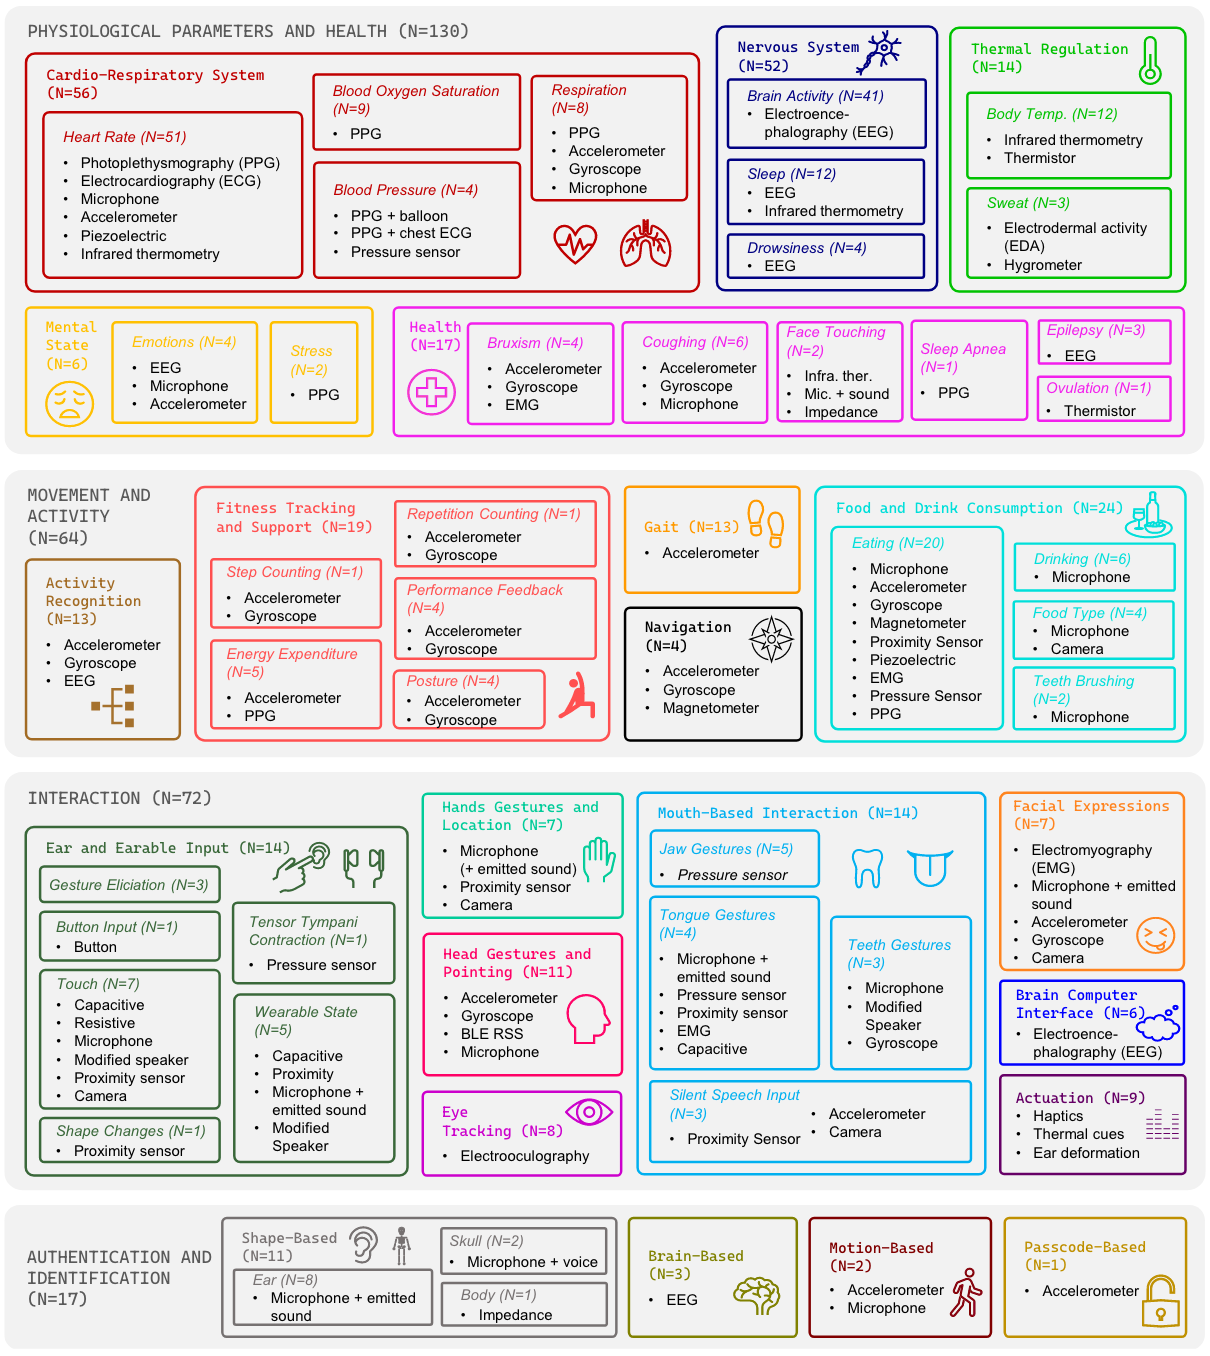
\includegraphics[scale=0.3525]{thesis-doc/images/sensing_with_earables_overview.png}
    \caption{Overview map of sensing with earables. The map displays all phenomena current research is about divided into the main four categories. For each phenomena, there is a number (N), which describes the available articles and all the used sensors used to detect these phenomena \cite{roddigerSensingEarablesSystematic2022a}.}
    \label{fig:sensing_with_earables_overview}
\end{figure}

\subsection{Physiological Monitoring and Health}
\label{Background:SensingWithEarables:Physiological}
The first categorical classification of sensing with earables is physiological parameters and health \cite{roddigerSensingEarablesSystematic2022a}.
The use of ear-worn sensors to track and maintain personal health by monitoring various physiological parameters is considered.
The parameters are categorized according to human body functions such as the cardio-respiratory system, nervous system, thermoregulation, mental status, and health monitoring.
The cardio-respiratory system is divided into the areas of heart rate, blood oxygen saturation, respiration, and blood pressure.
All these areas can be classified, for example, with a PPG (photoplethysmography). 
When determining the heart rate, a microphone, an accelerometer, an infrared thermometer, the piezoelectric, or an EEG (electrocardiography) can be used.
The nervous system includes the classification of brain activity, sleep, or drowsiness. 
All are determined using an EEG. When classifying sleep, an infrared thermometer can also be used for classification. 
The most researched area here in the context of earables is brain activity.
The third subcategory in the physiological parameters and health represents the mental state.
This has not yet been researched that far in the context of earables with 6 reference papers.
Emotions can be recognized using an EEG, a microphone, or an accelerometer, and even stress using a PPG.
Another subcategory is health which is divided into bruxism, coughing, face touching, sleep apnea, epilepsy, and ovulation.
Sensors such as an accelerometer, a gyroscope, a microphone, an EEG, PPG, or an infrared thermometer are used here.
For further details please refer to the original paper \cite{roddigerSensingEarablesSystematic2022a}.
The last part of the physiological parameters and health is thermal regulation. A distinction is made here between body temperature and perspiration. An EDA (electrodermal activity) and a hygrometer are used for sweating.
When classifying body temperature, an infrared thermometer, and a thermistor are used.
Due to the body temperature being the most crucial part of this thesis, this part will now be focused in more detail.

\paragraph{Body temperature}
\label{Background:SensingWithEarables:Physiological:BodyTemperature}
Bestbier and Fourie \cite{bestbierDevelopmentVitalSigns2018} applied the principle to a wearable form factor and achieved a small mean error of only $0.02$ $\pm$ $0.52 ^\circ C$. 
They used the TMP006 infrared sensor, which points directly at the tympanic membrane. 
The thermophilic voltage and the temperature sensor were made digitally available via hardware registers, from which the object temperature can be calculated. 
This reflects the temperature of the tympanic membrane after calibration.
However, the accuracy varies greatly between individual positions, which is attributed to the orientation of the sensor due to a wide variety of auditory canals.
This problem was solved by implementing intraparticipant calibration.
This should allow the sensor to self-calibrate automatically and improves the standard error by $56\%$ (from $0.5125 ^\circ C$ to $0.29 ^\circ C$) and the correlation coefficient from $0.4667$ to $0.8684$.

However, user-defined calibration is needed because the shape of the ear canal is different for each individual \cite{bestbierDevelopmentVitalSigns2018, luekenPhotoplethysmographybasedInearSensor2017, matsumotoEarbudtypeWearableHearable2019}.
Luken et al. integrated TI's TMP007 into the proposed measurement system to obtain information about human core temperature variation at a rate of $33 Hz$ \cite{luekenPhotoplethysmographybasedInearSensor2017}.
For individual calibration purposes, the voltage difference of the thermopile element and the chip temperature was transmitted in addition to the recorded object temperature.
However, the temperature was not further calibrated or processed in this work \cite{luekenPhotoplethysmographybasedInearSensor2017}.
Alternatively, surface skin temperature at the mastoid can be determined with high accuracy ($0.03 ^\circ C$ mean error) \cite{atallahErgonomicWearableCore2018}.
% TODO: read atallahErgonomicWearableCore2018 paper and insert content
A known factor for changes in body temperature is considered in earable research to be the response to external weather conditions \cite{barralonAugmentedHearingAssistance2015, boanoNoninvasiveMeasurementCore2013, celikEvaluationBehindtheEarECG2016} and during physical activities \cite{boanoNoninvasiveMeasurementCore2013, chagllae.MeasurementCoreBody2018, celikEvaluationBehindtheEarECG2016, matsumotoEarbudtypeWearableHearable2019, sugimotoDevelopmentWirelessSensing2011}.
% TODO: read all the previous papers and explain a lot more here!
These findings enable a number of applications that perform some important functions, such as alerting or vital signs and parameter tracking based on the identified relationships.
In addition, the relationship between body temperature recorded at the ear and ovulation (see subsection 4.5.6) and sleep (see subsection 4.2.2) has been demonstrated.
% TODO: remove the above sentence and insert content from sections mentioned

\subsection{Movement and Activity}
\label{Background:SensingWithEarables:Movement}
Another categorical classification of sensing with earables is movement and activity \cite{roddigerSensingEarablesSystematic2022a}.
Here, the focus is on detecting user movements and deriving insights about activities performed by the user. 
Movements detected at the ear can be classified into discrete classes, such as a user's posture, their movement, and also the type of activity. 
Beyond simply classifying sensor data, the project also explored how physical quantities can be derived from the user's movement to provide useful information for a variety of applications, including fitness tracking, gait analysis,
food and beverage consumption, and inertial navigation.
Most of the findings are recorded with the accelerometer and the gyroscope.
Activity recognition is recognized with it, but also with an EEG. Accelerometers and gyroscopes are also used as a basis for the fitness tracking and support subcategory, and the EEG for sensor performance.
When measuring the gait, the signal from the accelerometer is sufficient.
Significantly more sensors are used for classification when eating. While only one microphone signal was used for the drinking detection, a series of signals is used for the eating detection. 
Here the microphone, accelerometer, gyroscope, magnetometer, proximity sensor, piezoelectric, EMG, pressure sensor, and also the PPG is used.
When brushing teeth is detected, a microphone signal is evaluated.
In addition, the accelerometer and gyroscope signal as well as a magnetometer are also used for navigation.

\subsection{Interaction}
\label{Background:SensingWithEarables:Interaction}
Interaction is another categorical classification of sensing with earables \cite{roddigerSensingEarablesSystematic2022a}.
Since earables have a lot of different sensors, there are exciting possibilities for unique and novel interactions.
So far, attempts have been made to recognize inputs on the ear, but also on other parts of the body that can be recognized by sensors on the ear.
Subfields of interaction include ear or earable input, hand gestures or hand position, head gestures or orientations, eye tracking, mouth-based tracking, facial expressions, brain-computer interface, and actuation.
The most common tracking techniques are pressure or proximity sensors, accelerometer and gyroscope, the microphone, and EEG and EMG.
There are various input options for the ear-based or earable-based input. These include button inputs, touch or shape changes, and others.
Mouth-based interactions can be divided into jaw activities, tongue gestures, tooth activities, and silent speech input.

\subsection{Authentication and Identification}
\label{Background:SensingWithEarables:Authentication}
The final categorical classification of sensing with earables is authentication and identification \cite{roddigerSensingEarablesSystematic2022a}. 
For secure access to sensitive data, mobile devices often use biometrics such as fingerprints. 
Earable technologies have explored biometric authentication based on the unique ear, skull, or body features, as well as brain activity and body movement. 
Passcode-based authentication methods that use rhythmic patterns have also been proposed. 
The two main approaches are verification and identification, where performance is often measured using an equal error rate (ERR) to balance false acceptance and false rejection rates.
In this categorical classification, the microphone and emitted sound are used as the basis in shape-based authentication and identification on the ear, the microphone and voice are used in the skull, and impedance is used in the body.
The EEG is the basis for recognition in brain activity-based authentication and identification.
When the individual movement is used for authentication and identification, the accelerometer and the microphone are used, in the passcode-protected authentication and identification only the accelerometer signal is used.

\subsection{Sensing Platforms}
\label{Background:SensingWithEarables:SensingPlatforms}
Ear-based sensing platforms have gained considerable attention in the wearable technology field due to their potential for multiple applications and benefits. 
This chapter examines different types of ear-based sensor platforms, discusses their technical aspects and characteristics, captures their application, and examines the challenges and future directions in this field.
One type of ear-based sensor platform is the in-ear sensor, in which sensors are placed directly in the ear canal. Examples of in-ear sensors are earphones with integrated sensors that can monitor various physiological parameters \cite{maseHearablesNewPerspectives2020, bestbierDevelopmentVitalSigns2018, luekenPhotoplethysmographybasedInearSensor2017}. 
Another type is the on-ear sensor, which is placed on the outer ear or earlobe. 
These sensors can be in the form of clip-on devices or wearable ear accessories to collect specific data.
Behind-the-ear sensors represent another category of ear-based sensor platforms \cite{phamWAKEBehindtheearWearable2020, gilSmartWirelessEarWorn2019, biWearableSensorEating2017}.
These sensors are positioned behind the ear and are often found in hearing aids or smart ear tags. 
Finally, there are ear-worn wearables, which are wearable devices designed to be worn on the ear \cite{biWearableSensorEating2017, gilSmartWirelessEarWorn2019}. 
These include smart earbuds or earbuds that have sensors to monitor various health and activity-related metrics.
Technical aspects and features play a critical role in ear-based sensor platforms. 
Sensor technologies vary by platform, and each has its own advantages and limitations.
Connectivity and data transfer methods are essential for seamless integration with other devices or networks \cite{perezRecentAdvancesWearable2021}. 
Power management strategies are used to optimize battery life and ensure the longer use of ear-based sensor platforms \cite{nguyenInearBiosignalRecording2016}.
Ear-based sensor platforms find applications in various fields. 
In the area of health and wellness monitoring, these platforms enable the tracking of vital signs such as heart rate and body temperature \cite{roddigerRespirationRateMonitoring2020, atallahErgonomicWearableCore2018, maseHearablesNewPerspectives2020, rajbhandaryFeasibilityContinuousMonitoring2020a}.
They also facilitate the monitoring of sleep quality, stress levels, and other health-related parameters \cite{luekenPhotoplethysmographybasedInearSensor2017, wendtThermoregulationExerciseHeat2007}. 
In human-computer interaction, ear-based sensor platforms can serve as input modalities for gesture recognition or control interfaces, making them suitable for augmented reality, virtual reality, and gaming environments. 
In addition, ear-based biometrics are being explored for biometric identification and secure authentication purposes, offering an alternative to traditional authentication methods \cite{roddigerSensingEarablesSystematic2022a}.
Despite the potential benefits, ear-based sensor platforms face certain challenges. 
These include ensuring the accuracy and reliability of measurements, addressing convenience and usability concerns, and addressing privacy and data security issues \cite{bockAccuracyNewInfrared2005, roddigerRespirationRateMonitoring2020, bonziAccuracyPeripheralThermometers2016, gasimAccuracyTympanicTemperature2013, amoateng-adjepongAccuracyInfraredTympanic1999a, ericksonComparisonEarbasedBladder1993, chagllae.MeasurementCoreBody2018}. 
Future research and development efforts will focus on overcoming these challenges, exploring new applications, and advancing the capabilities of ear-based sensor platforms.
In summary, ear-based sensor platforms have emerged as promising tools in wearable technology. 
They offer a range of applications, from health monitoring to human-computer interaction to biometric authentication. 
By leveraging the unique properties of the ear, these platforms provide valuable insights and contribute to the advancement of wearable technology as a whole.

\paragraph{Earables: Temperature Measurement}
The research area of ear based temperature probing is not new territory.
% Temperature measurements at the eardrum
As early as 2010, infared tympanic thermometers (IRTTs) were used to compare temperature at the tympanic membrane with a rectal and oral sample \cite{bagleyValidityFieldExpedient2011, basakComparisonThreeDifferent2013, bhanguDetectionManagementHypothermia2010, fogtNoninvasiveMeasuresCore2017, ComparisonTwoMethods, kallmunzerLocalHeadNeck2011, muthInfraredEarThermometry2010, moran-navarroValiditySkinOral2019, leeValidityInfraredTympanic2011, keeneAccuracyTympanicTemperature2015}.
% TODO: write more if I have the time and fun.
% Temperature measurements outside the ear.
However, the tympanic membrane is not the only relevant measurement point in previous work. 
In 2018, Atallah et. al attached sensing devices to the mastoid to measure temperature \cite{atallahErgonomicWearableCore2018}. 
According to Atallah, skin temperature is easy to measure there, which is significantly different elsewhere on the body. 
Skin temperature differs by as much as $2 ^\circ C$ depending on the body position measured.
Atallah et. al placed 3 sensors on the lower area behind the ear, which was used to measure the heat flow for temperature.
In addition, the 3 sensors help to detect and eliminate potential measurement errors.
In this work, an 18 series thermistor from Murata was used to measure temperature.
% TODO: the determination of CBT is explained in more detail here, how to get there exactly, vllt potentially look more closely!
Also Nakada et. al have developed a method to measure temperature at the outer ear canal already in 2016 \cite{nakadaDevelopmentMethodEstimating2017a}.
Here, different positions on the external ear canal were measured to determine the temperature of the esophagus. 
The results showed that the temperature differed by about $ 1-2 ^\circ C$ from the comparative measurements at the tympanic membrane.
In addition, the variation in measurements at the external auditory canal is also significantly larger than the variation in measurements at the tympanic membrane $ \pm 0.78-2.82 ^\circ C$ \cite{nakadaDevelopmentMethodEstimating2017a}.
This is explained by the ambient temperature and other radiations.
With increasing ambient temperature and reduced radiation, the difference from the comparison measurement and also the fluctuations could be minimized.
However, the most commonly used measurement point on the ear for temperature is the tympanic membrane. 
The advantages of measuring temperature at the eardrum have already been explained in chapter \ref{Background:BodyTemperature:TemperatureMeasurements}.
Already in 2013, Boano et. al used the eardrum to measure temperature with an ear-based wearable \cite{boanoNoninvasiveMeasurementCore2013}. 
Here, the progression of temperature during a marathon run was tracked for the complete duration.
This has the advantage for the runner that knowing their temperature can help them perform better, get fewer injuries, and also reduce the risk of heart attacks.
The design was one of the biggest issues here, as the orientation of the sensor needs to be robust against strong physical movements.
In addition, there are constantly changing climatic conditions during a run that can potentially have a strong impact on the results.
A waiting period of at least 20 minutes was observed before the run to reduce fluctuations and erroneous readings \cite{chagllae.MeasurementCoreBody2018}.
During the measurement, there was an initial drop in temperature at the beginning of the run, and only then was there an increase in body temperature, as also expected.
The drop was explained by the wind conditions present there.
In addition, there was considerable loss of data during the marathon, which together with the cold outside temperatures led to massive influences. 
In the end, this resulted in few dependencies among the test subjects.
Also considered were the temperature conditions that prevailed on site. 
After the end of the run, the temperature dropped back to normal.
In addition to the temperature observation of the marathon run, the temperature was also observed over a whole day \cite{boanoNoninvasiveMeasurementCore2013}.
Body temperature is significantly lower at night than during the day, even with nearly $1 ^\circ C$ difference at peak.
Other increases in temperature were detected during eating (about $0.4 ^\circ C$) and when the outside temperature was $0 ^\circ C$ during walking.
Another work that looks at measuring the temperature at the tympanic membrane was Bestbier in 2018 \cite{bestbierDevelopmentVitalSigns2018}.
Bestbier has developed a wearable that uses a self-built device on the ear to measure temperature with an infrared sensor (TMP006) pointed at the tympanic membrane.
The rest of the components were attached to a headband, such as the battery and also the computing units.
Accuracy varies significantly from person to person due to different ear canals.
However, Bestbier has solved this with an in-person calibration by having the sensor self-calibrate.
This improves the standard error by $56\%$ from $0.5125 ^\circ C$ to $0.29 ^\circ C$. The interclass correlation coefficient (ICC) also improves from $0.4667$ to $0.8684$.
Lueken designed an earplug in 2017 that also measures temperature using an infrared sensor on the eardrum \cite{luekenPhotoplethysmographybasedInearSensor2017}.
In addition to temperature, ACC and PPG were also measured.
However, the ACC signal was used to optimize the PPG signal rather than the temperature signal. 
This is to make the signal resistant to head motion.
Lueken integrated TI's TMP007 into his system to obtain information about variations in human core temperature. 
Here, the temperature was recorded at $33 Hz$.
For individual calibration purposes, the voltage difference between the thermopile element and the chip temperature was recorded in addition to the acquired object temperature.
In another study in 2018, Chaglla E. et. al looked at developing a novel sensor to measure core body temperature \cite{chagllae.MeasurementCoreBody2018}. 
The sensor is based on a graphene-inked infrared thermopile sensor positioned on the eardrum. 
The graphene coating on the active surface of the sensor improves sensitivity and performance. 
The measurement principle is based on the acquisition of electrical signals from the sensor.
Two different studies were conducted in this regard. 
In addition to a laboratory study, a field study with physical activity was also conducted.
In the laboratory study, seated and resting test subjects were examined for a period of 10 minutes at 60 seconds using a total of four different devices. 
The in-house device with the graphene-inked thermopile sensor and an infrared drum thermometer (IRTT) ThermoScan 7 Age Precision-IRT6520 (Braun GmbH, Kronberg, Germany) were referenced.
In the field study, a 26-year-old man was examined during activity on a cross-trainer in an outdoor gym. The measurements lasted 25 minutes and took place on a cloudy day at a temperature of 21 degrees Celsius. 
Additionally, the temperature information of the cross trainer was recorded as well, the Cosinuss One (Cosinuss GmbH, Munich, Germany) was used for this purpose.
The results showed that the graphene-inked thermopile sensor measurements provided better results than the Cosinuss One \cite{chagllae.MeasurementCoreBody2018}. 
The latter seemed to be more sensitive to external parameters. 
It was noted that the sensors were very comfortable during wear. 
Additionally, it was observed that the sensors required a calibration period at the beginning and provided relevant measurement results after about 8 minutes. 
However, in the laboratory study, the measurements were taken only for a period of 10 minutes.
In another work, the temperature at the ear was also measured in 2020 \cite{chenInearThermometerWearable2020}.
Here, an infrared sensor also recorded the temperature. 
The focus of this work was to design a wearable device that can be worn over a longer period of time. 
Here the focus was on size, weight, and battery life.
An app was also developed to transfer the data.
The ground truth is a conventional thermometer on the ear.
During activities, the results were 0.15 degrees below those of ground truth, but this is explained by the presence of sweat.
The range of error was $\pm 0.16 ^\circ C$.
The correlation is $0.9438$, and the average accuracy is $99\%$.

% OpenEarable
\paragraph{OpenEarable Platform}
\label{Background:SensingWithEarables:OpenEarable}
The OpenEarable serves as the core sensing platform for this thesis. 
It is an open source hardware and software platform for the development of multisensory audible devices, originally introduced by Röddiger et al. in 2021 \cite{roddigerOpenEarableOpenHardware2022}. 
The OpenEarable was developed at KIT and enables rapid prototyping and exploration of novel earable applications. 
It was not developed as a finished product, but serves as a platform for future projects.

The OpenEarable hardware design is based on the Arduino Nano33 BLE, which includes the Bluetooth SoC nRF52840 from Nordic Semiconductor.
This chip integrates a 32-bit ARM Cortex M4F processor with 256 KB of RAM and supports Bluetooth 5.4 connectivity. 
For audio detection, the OpenEarable features a high-performance STMicroelectronics LSM6DSRTR low-power digital microphone. 
This enables high dynamic range audio sampling up to 44 kHz. 
Motion and orientation tracking is provided by the 9-axis inertial measurement unit (IMU), which combines a 3-axis gyroscope, a 3-axis accelerometer and a 3-axis magnetometer. 
In addition, a push button and a controllable LED are built into the circuit board.
In addition to the main circuit board, an earpiece has also been designed. 
This also features an ear canal pressure and temperature sensor, an inward-facing ultrasonic microphone, and a speaker.
However, the earpiece was not used in the context of this master thesis
Finally, a rechargeable 90 mAh lithium-ion polymer battery powers the platform.
This combination of sensors enables the OpenEarable device to collect and analyze audio, motion, environmental, and biometric data in real time. The nRF52840 SoC also provides sufficient processing capabilities for integrated machine learning inferencing. 
Multiple peripherals can also be connected via the available GPIOs and I2C bus. 
An integrated microSD card slot enables storage and buffering of sensor data.
By building on the OpenEarable hardware and software architecture, the development time to create a custom multimodal ear sensing device can be dramatically reduced compared to designing a new platform from scratch. 

OpenEarable can be used for a variety of applications, such as health monitoring, authentication, identification and human-computer interaction.
The platform is still under development, but has the potential to be used for a wide range of applications. 
OpenEarable's capabilities for rapid prototyping, flexible extension, and sensor fusion were key enablers for the research presented in this paper.
% TODO: reference the chapter for more details on the general interaction of all components, how everything works together.

% https://media.digikey.com/pdf/Data%20Sheets/Excelitas%20PDFs/TPiS_1S_1385.pdf

% address translator weiter hinten, wo ich die implementierung ändere
% \subsection{Address translator}
% da die sensoren alle die gleiche addresse haben werden brauche wir da noch so address übersetzter, ich denke sopwas in die richung: 
% https://www.analog.com/media/en/technical-documentation/data-sheets/4316fa.pdf